Jets originating from the fragmentation of $b$-quarks are often referred to as $b$-jets and can be distinguished from lighter quarks due to its relatively long lifetime and large mass. When a $b$-quark decays, it typically transitions into a $c$-quark which is a second generation quark. This decay is suppressed by the CKM matrix, resulting in a measurable displacement between the PV and the decay vertex of the $b$-jet of up to several millimeters, and can be seen in Figure~\ref{fig:reco_btagged_jet}.

\begin{figure}[htbp]
  \centering
  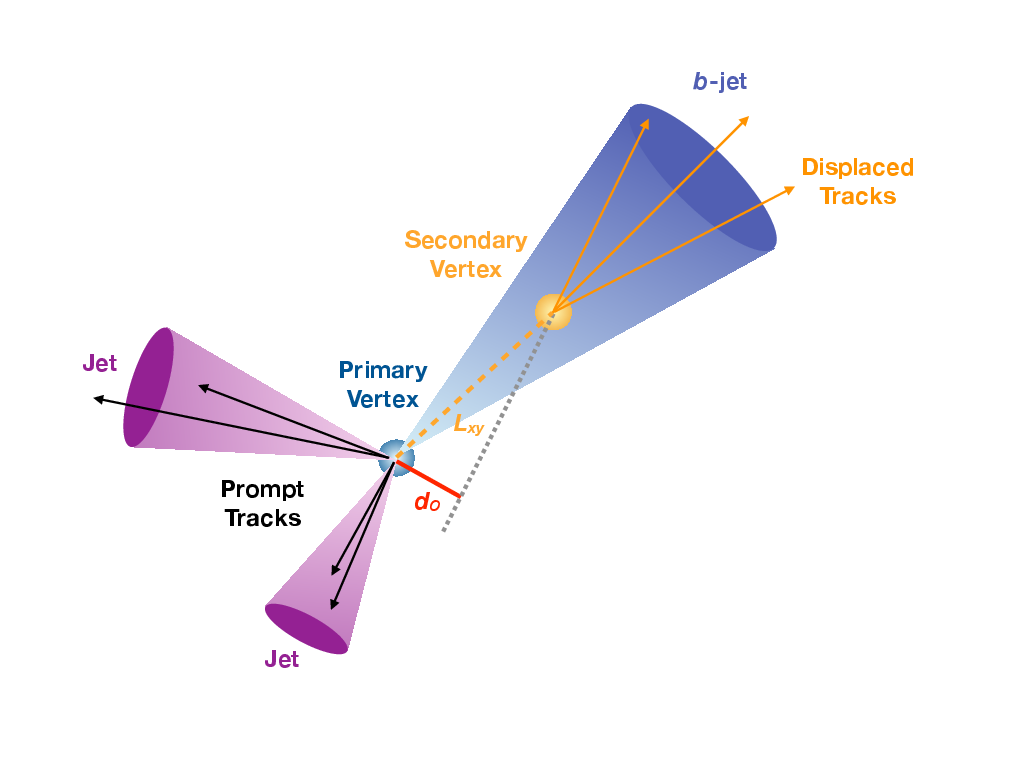
\includegraphics[width=0.6\textwidth]{figures/reco/reco_btagged_jet.png}
  \caption{A $b$-jet with a secondary vertex displaced from the primary vertex. Taken from Ref.~\cite{ATLAS:2021piz}.}\label{fig:reco_btagged_jet}
\end{figure}

Previously, $b$-jet identification was performed via a multivariate algorithm that produced a discriminant on how likely a given jet originates from $b$-quark fragmentation, as opposed to a lighter parton. Several of these algorithms have been developed, with the most prominent being DL1~\cite{dl1_paper} which is a feed-forward neural network. For Run 3 however, DL1 has been superseded by GN2~\cite{Duperrin:2023elp}, a graph neural network (GNN) based tagger. This tagger significantly improves on DL1 with up to four times better background rejection relative to the DL1 taggers as seen in Figure~\ref{fig:reco_gn2_performance}.

\begin{figure}[htbp]
  \centering
  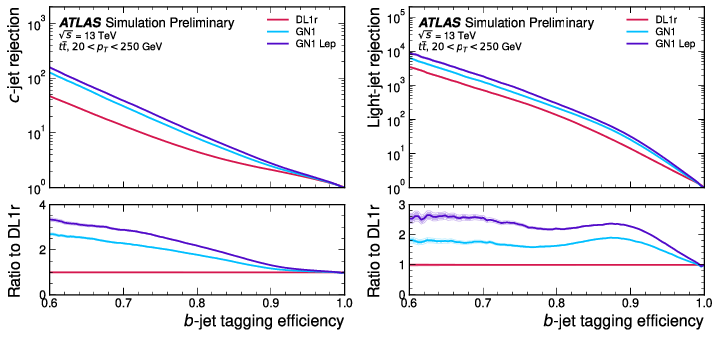
\includegraphics[width=0.8\textwidth]{figures/reco/reco_gn2_performance.png}
  \caption{Comparison of the GN2 tagger performance with respect to the previous DL1 tagger. Taken from Ref.~\cite{Duperrin:2023elp}.}\label{fig:reco_gn2_performance}
\end{figure}

To accommodate the varying needs of different analyses, a series of $b$-tagged WPs are supported, each defined by specific $b$-tagging efficiency as measured in $t\bar{t}$ events. The supported working points consists of a $65\%$, $70\%$, $77\%$, $85\%$ and $90\%$. Additionally, GN2 supports $c$-jet identification although this is not used in this thesis and will not be discussed further.